%%%%%%%%%%%%%%%%%%%%%%%%%%%%%%%%%%%%%%%%%%%%%%%%%%%%%%%%%%%%%%%%%%%%%%%%%%%%%%%%
% TUM-Vorlage: Wissenschaftliche Arbeit
%%%%%%%%%%%%%%%%%%%%%%%%%%%%%%%%%%%%%%%%%%%%%%%%%%%%%%%%%%%%%%%%%%%%%%%%%%%%%%%%
%
% Rechteinhaber:
%     Technische Universität München
%     https://www.tum.de
% 
% Gestaltung:
%     ediundsepp Gestaltungsgesellschaft, München
%     http://www.ediundsepp.de
% 
% Technische Umsetzung:
%     eWorks GmbH, Frankfurt am Main
%     http://www.eworks.de
%
%%%%%%%%%%%%%%%%%%%%%%%%%%%%%%%%%%%%%%%%%%%%%%%%%%%%%%%%%%%%%%%%%%%%%%%%%%%%%%%%

%%%%%%%%%%%%%%%%%%%%%%%%%%%%%%%%%%%%%%%%%%%%%%%%%%%%%%%%%%%%%%%%%%%%%%%%%%%%%%%%
\documentclass[%
    fontsize=11pt, % Schriftgröße
    twoside=off % kein einseitiges Layout
]{scrbook} % Dokumentenklasse: KOMA-Script Book
\usepackage{scrlayer-scrpage} % Anpassbare Kopf- und Fußzeilen

\usepackage[utf8]{inputenc} % Textkodierung: UTF-8
\usepackage[T1]{fontenc} % Zeichensatzkodierung

\usepackage[ngerman]{babel} % Deutsche Lokalisierung
\usepackage{graphicx} % Grafiken

% Schriftart Helvetica:
\usepackage[scaled]{helvet}
\renewcommand{\familydefault}{\sfdefault}

% Silbentrennung:
\usepackage{hyphenat}
\hyphenation{TUM in-te-res-siert} % Eigene Silbentrennung
%\tolerance 2414
%\hbadness 2414
%\emergencystretch 1.5em
%\hfuzz 0.3pt
%\widowpenalty=10000     % Hurenkinder
%\clubpenalty=10000      % Schusterjungen
%\vfuzz \hfuzz

\usepackage[hidelinks]{hyperref} % Hyperlinks
\usepackage[onehalfspacing]{setspace} % 1,5facher Zeilenabstand
\usepackage{calc} % Berechnungen
\usepackage{enumitem} % Mehr Kontrolle über itemize-, enumerate- und description-Umgebungen
\usepackage{relsize} % Schriftgröße in Abhängigkeit von aktueller anpassen
\usepackage{tabularx} % Flexiblere Tabellen
\usepackage[tablewithout, figurewithout]{caption} % Anpassen von Beschriftungen

% Nummerierung von Abbildungen & Tabellen durchgängig, statt nach Kapiteln:
\usepackage{chngcntr}
\counterwithout{figure}{chapter}
\counterwithout{table}{chapter}

% Abkürzungen, Glossare:
\usepackage[%
    xindy,% xindy zum Indexieren verwenden
    acronym,% Separates Akronym-Verzeichnis
    nopostdot,% Kein Punkt am Ende einer Beschreibung im Glossar
]{glossaries}

% Spezielle Befehlsdefinitionen:
\newcommand{\Thema}{}

% Debugging:
%\usepackage{showframe} % Layout-Boxen anzeigen
%\usepackage{layout} % Layout-Informationen
%\usepackage{printlen} % Längenwerte ausgeben
 % !!! NICHT ENTFERNEN !!!
%%%%%%%%%%%%%%%%%%%%%%%%%%%%%%%%%%%%%%%%%%%%%%%%%%%%%%%%%%%%%%%%%%%%%%%%%%%%%%%%

\renewcommand{\Thema}{%
    Thema der Arbeit (optional)}

%%%%%%%%%%%%%%%%%%%%%%%%%%%%%%%%%%%%%%%%%%%%%%%%%%%%%%%%%%%%%%%%%%%%%%%%%%%%%%%%
%%%%%%%%%%%%%%%%%%%%%%%%%%%%%%%%%%%%%%%%%%%%%%%%%%%%%%%%%%%%%%%%%%%%%%%%%%%%%%%%
% EINSTELLUNGEN
%%%%%%%%%%%%%%%%%%%%%%%%%%%%%%%%%%%%%%%%%%%%%%%%%%%%%%%%%%%%%%%%%%%%%%%%%%%%%%%%

\KOMAoptions{parskip=full}


% Seitenränder:

\newcommand{\SeitenrandOben}{25.8mm}
\newcommand{\SeitenrandRechts}{21mm}
\newcommand{\SeitenrandLinks}{40mm}
\newcommand{\SeitenrandUnten}{24.8mm}
\newcommand{\FusszeileHoehe}{11.7mm}

\usepackage[a4paper,
    head=0pt,
    top=\SeitenrandOben,
    bottom=\SeitenrandUnten,
    inner=\SeitenrandLinks,
    outer=\SeitenrandRechts
]{geometry}


% Fußzeilen:

\setlength{\footheight}{\FusszeileHoehe}
\clearscrheadfoot
\ifoot*{\Thema\vfill}
\ofoot*{\pagemark\vfill}
\setkomafont{pageheadfoot}{\fontsize{9pt}{13pt}\normalfont}
\setkomafont{pagefoot}{\bfseries}
\setkomafont{pagenumber}{\normalfont}
\pagestyle{scrheadings}


% Fußnoten:

\KOMAoptions{%
    footnotes=multiple % mehrere Fußnoten werden durch Zeichen getrennt
}
%\setfootnoterule[.6pt]{5.08cm}
\renewcommand{\footnoterule}{\hrule width 5.08cm height .6pt \vspace*{3.9mm}}
%\setlength{\footnotesep}{5mm}
\deffootnote{2mm}{2mm}{%
    \makebox[2mm][l]{\textsuperscript{\thefootnotemark}}%
}
\setkomafont{footnoterule}{\fontsize{9pt}{20pt}\selectfont}


% Überschriften:

\KOMAoptions{%
    open=any, % keine Festlegung auf linke oder rechte Seite
    numbers=noendperiod, % kein automatischer Punkt nach Gliederungsnummer
    headings=small
}

\makeatletter
\g@addto@macro{\@afterheading}{\vspace{-\parskip}} % \parskip nach Gliederungsbefehlen entfernen
\renewcommand*{\chapterheadstartvskip}{\vspace{\@tempskipa}\vspace{-3pt}} % Korrektur für Abstand über Kapitelüberschriften
\makeatother

\setkomafont{disposition}{\normalfont\sffamily}

\setkomafont{chapter}{\normalfont\fontsize{19pt}{22pt}\selectfont}
\RedeclareSectionCommand[%
  beforeskip=0pt,
  afterskip=29pt
]{chapter}
\renewcommand*{\chapterformat}{\thechapter.\enskip} % Immer Punkt nach Kapitelnummer

\setkomafont{section}{\fontsize{15pt}{17pt}\selectfont}
\RedeclareSectionCommand[%
  beforeskip=0pt,
  afterskip=24.1pt
]{section}
\renewcommand*{\sectionformat}{\makebox[13mm][l]{\thesection.\enskip}} % Feste Breite für Abschnittsnummer und immer Punkt danach

\setkomafont{subsection}{\bfseries\fontsize{12pt}{13pt}\selectfont}
\RedeclareSectionCommand[%
  beforeskip=0pt,
  afterskip=1pt
]{subsection}
\renewcommand*{\subsectionformat}{\makebox[13mm][l]{\thesubsection.\enskip}} % Feste Breite für Unterabschnittsnummer und immer Punkt danach


% Listen:

\setlist{%
    labelsep=0mm,
    itemindent=0pt,
    labelindent=0pt,
    align=left,
    parsep=1.5ex
}
\setlist[itemize]{%
    leftmargin=5mm,
    labelwidth=4.9mm
}
\setlist[itemize,1]{%
    before={\vspace{0.25ex}},
    label={\raisebox{.35ex}{\smaller[2]\textbullet}},
    after={\vspace{-\parsep}\vspace{-.25ex}}
}
\setlist[itemize,2]{%
    label={\raisebox{.35ex}{\rule{.58ex}{.58ex}}}
}
\setlist[enumerate]{%
    leftmargin=10mm,
    labelwidth=9.9mm
}
\setlist[enumerate,2]{%
    label={\alph*.}
}

\setlist[description]{%
%    labelindent=!,
    leftmargin=1em,
    labelwidth=!,
    parsep=0mm,
    partopsep=0mm,
    labelsep=1em,
}


% Verzeichnisse:

\KOMAoptions{%
    toc=flat, % keine Einrückungen im Inhaltsverzeichnis
    toc=chapterentrydotfill, % Punkte bis zur Seitennummer bei Kapiteln
    listof=entryprefix, % Präfix für Einträge in Abbildungs- und Tabellenverzeichnis
    listof=nochaptergap, % Kein Abstand für Kapiteleinträge in extra Verzeichnissen
}

\makeatletter
\renewcommand{\@dotsep}{.3} % Abstand der Füllpunkte

% "chapteratlist" für Inhaltsverzeichnis auswerten:
\renewcommand*{\addchaptertocentry}[2]{%
  \Iftocfeature{toc}{chapteratlist}{}{%
    \addtocontents{toc}{\protect\vspace{-10pt}}% extra Abstand vor Kapitelüberschriften in Inhaltsverzeichnis entfernen
  }%
  % Originaldefinition aus scrbook.cls:
  \addtocentrydefault{chapter}{#1}{#2}%
  \if@chaptertolists
    \doforeachtocfile{%
      \Iftocfeature{\@currext}{chapteratlist}{%
        \addxcontentsline{\@currext}{chapteratlist}[{#1}]{#2}%
      }{}%
    }%
    \@ifundefined{float@addtolists}{}{\scr@float@addtolists@warning}%
  \fi%
}
\makeatother

\AfterTOCHead[toc]{\protect\vspace{.8ex}} % Abstand zwischen Überschrift und Inhaltsverzeichnis
\setuptoc{toc}{noparskipfake} % Angleichung der Abstände nach Inhaltsverzeichnisüberschrift an andere Überschriften
\unsettoc{toc}{chapteratlist} % kein Abstand vor Kapiteleinträgen im Inhaltsverzeichnis, funktioniert nur durch obige Redefinition von \addchaptertocentry

% -- Abbildungs- und Tabellenverzeichnis:

\AfterTOCHead[lof]{\protect\vspace{-.1ex}\doublespacing} % Abstand zwischen Überschrift und Abbildungsverzeichnis, doppelter Zeilenabstand
\setuptoc{lof}{noparskipfake} % Angleichung der Abstände nach Abbildungsverzeichnisüberschrift an andere Überschriften

\AfterTOCHead[lot]{\protect\vspace{-.1ex}\doublespacing} % Abstand zwischen Überschrift und Tabellenverzeichnis, doppelter Zeilenabstand
\setuptoc{lot}{noparskipfake} % Angleichung der Abstände nach Tabellenverzeichnisüberschrift an andere Überschriften

% Beschriftungen:
\DeclareCaptionFormat{WissenschaftlicheArbeiten}{\fontsize{8pt}{10pt}\selectfont#1 #2#3\par}
\DeclareCaptionLabelFormat{WissenschaftlicheArbeiten}{\bfseries\selectfont#1 #2}

% -- Tabellen:
\captionsetup[table]{%
    format=WissenschaftlicheArbeiten,
    labelformat=WissenschaftlicheArbeiten,
    labelsep=none,
    singlelinecheck=off,
    justification=raggedright,
    skip=3pt
}

% -- Abbildungen:
\captionsetup[figure]{%
    format=WissenschaftlicheArbeiten,
    labelformat=WissenschaftlicheArbeiten,
    labelsep=none,
    singlelinecheck=off,
    justification=raggedright,
    skip=6.6mm
}


% Tabellen:
\renewcommand{\arraystretch}{1.8} % Skalierung der Tabellen
\newcolumntype{M}{X<{\vspace{4pt}}} % Spaltentyp mit Abstand rechts


% Glossare & Abkürzungsverzeichnis:

\makeglossaries
\newacronym{abk}{Abk.}{Abkürzungen}
\newacronym{bez}{Bez.}{Bezeichnung}
\setacronymstyle{short-long}

\makeatletter
\newlength{\@glsdotsep}
\setlength{\@glsdotsep}{\@dotsep em}
\newcommand*{\glsdotfill}{\leavevmode \cleaders \hb@xt@ \@glsdotsep{\hss .\hss }\hfill \kern \z@}
\makeatother

\newglossarystyle{WissenschaftlicheArbeiten}{%
  \setglossarystyle{index}%

  \renewcommand*{\glossaryheader}{\vspace{.75em}}%
  \renewcommand*{\glstreenamefmt}[1]{##1}%
  \renewcommand*{\glossentry}[2]{%
     \item\glsentryitem{##1}\glstreenamefmt{\glstarget{##1}{\glossentryname{##1}}}%
     \ifglshassymbol{##1}{\space(\glossentrysymbol{##1})}{}%
     \space-\space\glossentrydesc{##1}\glsdotfill\glspostdescription\space ##2%
  }%
  \renewcommand*{\glsgroupheading}[1]{%
    \item\glstreenamefmt{\textbf{\fontsize{14}{17}\selectfont\enskip\glsgetgrouptitle{##1}}}\vspace{.3em}}%
}

\setglossarystyle{WissenschaftlicheArbeiten}


 % !!! NICHT ENTFERNEN !!!
%%%%%%%%%%%%%%%%%%%%%%%%%%%%%%%%%%%%%%%%%%%%%%%%%%%%%%%%%%%%%%%%%%%%%%%%%%%%%%%%
\usepackage{amsmath}


\begin{document}

\title{Reconstruction of suspended sediment using artificial intelligence}
\author{Dominic Mutzhas}
\date{Datum}
%\maketitle   %also das brauchen wir nicht wegen dem deckblatt

\tableofcontents % Inhaltsverzeichnis

\chapter{Introduction}

\section{}

\subsection[]{Absatzüberschrift}
Accurate suspended sediment modeling is needed for a variety of reasons. One example is the planning of hydraulic river structures like water reservoirs, where the slowing of the water leads to a deposition of suspended sediment, and eventually to complete aggradation. 

Since the interaction between hydraulic structures and the environment is very complex, any available data in that flied is important, and supended sediment data can be helpful in evaluating the impact of hydraulic structures on ecosystems.
Predicting these much needed values turns out to be a difficult problem, since Erosion and sediment transport are very physically complex phenomena. Thus the accuracy of physical models is also limited, since The large number of [obscure] parameters involved, requires many assumptions and simplifications to be made.

This difficulty has lead to the development of data driven methods,where the rivers suspended sediment dynamic is approximated with a model which is built directly from the data. One big advantage with these methods is that the data implicitely represents the physical phenomena, and thus allow modeling, without requiring any knowlege about the actualy physical theory. 
A very simple type of a data driven Models is the classic power function \gls{src} \cite{Jansson}:
%----------------------------------------
\begin{equation}\label{eq:emc}
Qs=aQ^{b}
\end{equation}   
%---------------------------------------
where a and b are regression parameters that describe the relationship between the suspended sediment transport \textit{Qs} and the flow \textit{Q}.\cite{afan2016past}

 Though very commonly used, more and more evidence which suggest that these classic \gls{src} are not only not a very good solution for this problem, but also that there are much better solutions availiable. \cite{past}




As the machine learning(ML) revolution progresses, more and more scientific disciplines are trying to take advantage of it's strenghts in handling complex and non-linear problems. As such it has also found it's way into the field of water management in the form of artificial neural networks (ANN), especially for the prediction of Flow and suspended Sediment.


\begin{figure}[!ht]
\noindent\hspace{0.5mm}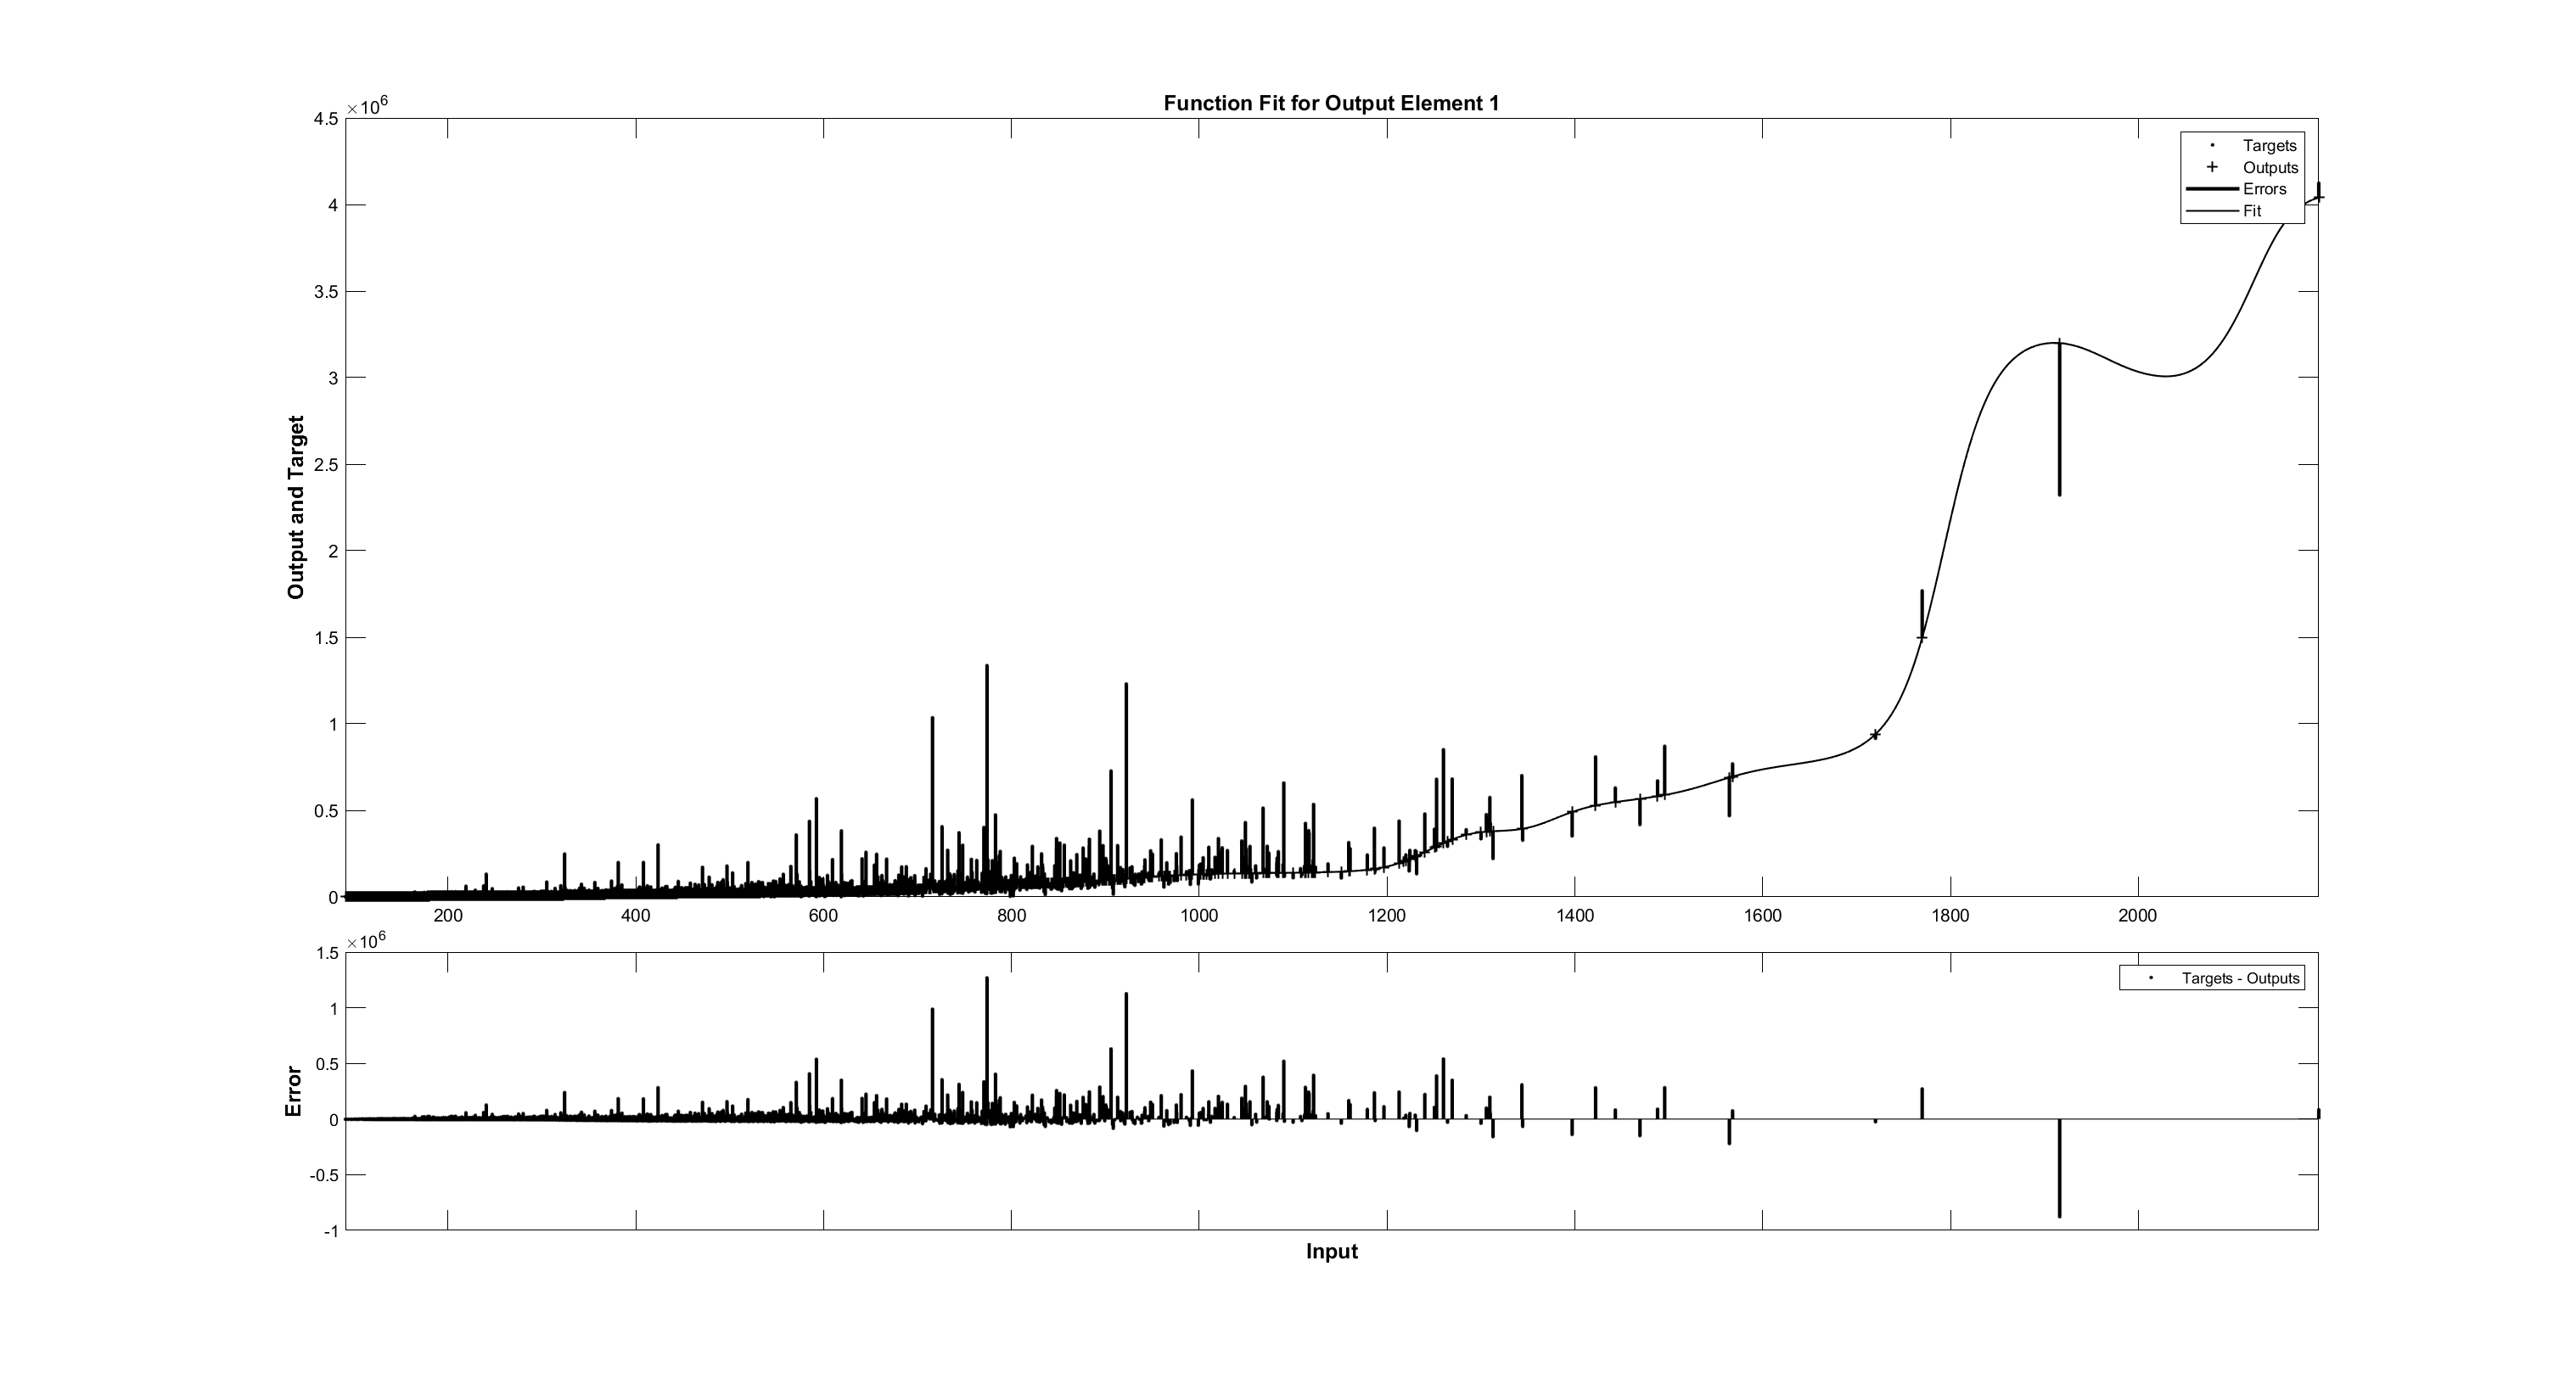
\includegraphics[width=12cm]{./Ressourcen/plots/overfitting_11_11}
\caption{Titel, Autor}
\end{figure}

\clearpage

Passen Sie gegebenenfalls die Ränder an die Vorgaben Ihres Prüfers an und
beachten Sie dabei, dass das Logo der TUM sich oben rechts innerhalb der
Ränder, auf der Titelseite befindet. Für die Titelseiten stehen separate
Vorlagen zur Verfügung.

Zur Definition von \gls{abk} erstellen Sie für die gewünschte Abkürzung einen
Eintrag in der Datei \texttt{Abkuerzungen.tex} und referenzieren sie ihn
mittels \texttt{\textbackslash{}gls}; diese tauchen nach einem Lauf mit
\texttt{latexmk} im Abkürzungsverzeichnis auf. Beispiel:

\vspace{-\baselineskip}
\begin{description}[leftmargin=1em+5mm, labelindent=5mm]
\item[Definition in \texttt{Abkuerzungen.tex}:] \texttt{\textbackslash{}newacronym\{abk\}\{Abk.\}\{Abkürzungen\}\}}
\item[Referenzierung:] \texttt{\textbackslash{}gls\{abk\}}
\end{description}

Für weitere Informationen zu Glossaren und Abkürzungen siehe die Dokumentation
des Pakets \texttt{glossaries} und die entsprechenden Abschnitte in den
Vorlagendateien.


\subsection[]{Aufzählungen}

\begin{itemize}
\item Dies ist die Standardaufzählung
    \begin{itemize}
    \item Dies ist die nächste Ebene der Aufzählung
    \end{itemize}
\end{itemize}


\subsection[]{Nummerierungen}

\begin{enumerate}
\item Erster Punkt der Nummerierungen
    \begin{enumerate}
    \item Unterpunkt der Nummerierungen
    \end{enumerate}
\end{enumerate}
\clearpage

\listoffigures % Abbildungsverzeichnis

\printacronyms[title={Abkürzungsverzeichnis}] % Abkürzungsverzeichnis

\listoftables % Tabellenverzeichnis

\onehalfspacing

\addchap{Tabellenvarianten}

\vspace{22mm}
\section*{Überschrift Tabelle 1}

\begin{table}[!h]
\begin{tabularx}{\textwidth + 5pt}{@{\hspace{3pt}} M | @{\hspace{3pt}} M}
\multicolumn{2}{@{}X}{%
    \begin{tabularx}{\textwidth}{@{\hspace{3pt}} M @{\hspace{14.5pt}} M}
    \textbf{Spalte 1} & \textbf{Spalte 2}
    \end{tabularx}%
} \\
\hline
Nummer 1 & Nummer 2 \\
\hline
Nummer 1 & Nummer 2 \\
\hline
Nummer 1 & Nummer 2 \\
\hline
\end{tabularx}

\caption{Beschreibung}
\end{table}


\vspace{\parskip}
\section*{Überschrift Tabelle 2}

\begin{table}[!h]
\hspace{-5pt}
\begin{tabularx}{\textwidth + 5pt}{| @{\hspace{3pt}} M | @{\hspace{3pt}} M |}
\hline
\textbf{Spalte 1} & \textbf{Spalte 2} \\
\hline
Nummer 1 & Nummer 2 \\
\hline
Nummer 1 & Nummer 2 \\
\hline
Nummer 1 & Nummer 2 \\
\hline
\end{tabularx}
\caption{}
\end{table}


\vspace{\parskip}
\section*{Überschrift Tabelle 3}

\begin{table}[!h]
\begin{tabularx}{\textwidth}{@{} M M}
\textbf{Spalte 1} & \textbf{Spalte 2} \\
Nummer 1 & Nummer 2 \\
Nummer 1 & Nummer 2 \\
Nummer 1 & Nummer 2 \\
\end{tabularx}
\caption{}
\end{table}

\clearpage

\addchap{Tabellenvarianten 2}

\vspace{22mm}
\section*{Überschrift Tabelle 1}

\begin{table}[!h]
\fontsize{9pt}{13pt}\selectfont
%\renewcommand{\arraystretch}{1.8}
\hspace{-5pt}
\begin{tabularx}{\textwidth + 5pt}{@{\hspace{3pt}} M | @{\hspace{3pt}} M}
\multicolumn{2}{@{}X}{%
    \begin{tabularx}{\textwidth}{@{\hspace{3pt}} M @{\hspace{14.5pt}} M}
    \textbf{Spalte 1} & \textbf{Spalte 2}
    \end{tabularx}%
} \\
\hline
Nummer 1,\newline\,mehrzeilig in Schriftgröße 9 pt & Nummer 2 \\
\hline
Nummer 1 & Nummer 2 \\
\hline
Nummer 1 & Nummer 2 \\
\hline
\end{tabularx}

\caption{}
\end{table}


\vspace{\parskip}
\section*{Überschrift Tabelle 2}

\begin{table}[!h]
\fontsize{9pt}{13pt}\selectfont
\hspace{-5pt}
%\renewcommand{\arraystretch}{1.8}
\begin{tabularx}{\textwidth + 5pt}{| @{\hspace{3pt}} M | @{\hspace{3pt}} M |}
\hline
\textbf{Spalte 1} & \textbf{Spalte 2} \\
\hline
Nummer 1 & Nummer 2 \\
\hline
Nummer 1 & Nummer 2 \\
\hline
Nummer 1 & Nummer 2 \\
\hline
\end{tabularx}
\caption{}
\end{table}


\vspace{\parskip}
\section*{Überschrift Tabelle 3}

\begin{table}[!h]
\fontsize{9pt}{13pt}\selectfont
%\renewcommand{\arraystretch}{1.8}
\begin{tabularx}{\textwidth}{@{} M M}
\textbf{Spalte 1} & \textbf{Spalte 2} \\
Nummer 1 & Nummer 2 \\
Nummer 1 & Nummer 2 \\
Nummer 1 & Nummer 2 \\
\end{tabularx}
\caption{}
\end{table}
% -------------------------------------------------------------------
% add bibliography-related commands here 
\bibliographystyle{plain}
\bibliography{bibfile_wa}   
\end{document}
